\documentclass[draft]{agujournal2018}
\usepackage{apacite}
\usepackage{url} %this package should fix any errors with URLs in refs.
\usepackage{lineno}
\linenumbers

\draftfalse
\journalname{JGR: Earth Surface}

%% you probably have to kill these custom commands later %% 
\newcommand\be{\begin{equation}} % shortcut to start eq envs 
\newcommand\ee{\end{equation}}   % shortcut to end eq envs
\newcommand\bra{\langle}
\newcommand\ket{\rangle}
\usepackage{amsmath,amssymb,amsfonts,amsthm}
\usepackage{comment}
\usepackage{wrapfig}
\usepackage{lipsum}
\usepackage{booktabs} % for wrapping text around tabulars in accord with
% https://tex.stackexchange.com/questions/49300/wrap-text-around-a-tabular

\begin{document}

\title{Joint stochastic theory of fluvial bedload transport and bed elevation changes deriving heavy-tailed sediment resting times}
\authors{James K. Pierce\affil{1}\thanks{Vancouver, British Columbia, Canada}, and Marwan A. Hassan\affil{1}\thanks{Vancouver, British Columbia, Canada}}
\affiliation{1}{Department of Geography, University of British Columbia}
\correspondingauthor{James K. Pierce}{kpierce@alumni.ubc.ca}

\begin{keypoints}
\item We model fluvial bedload activity and local bed elevation as a two-species stochastic birth-death process.
\item Resulting timescales of sediment storage by burial lie on heavy-tailed power-law distributions.
\item These distributions have universal characteristics, offering a possibility of discriminating the signature of burial in tracer experiments.
\end{keypoints}

\begin{abstract}
A consensus has formed that fluvial bedload transports with heavy-tailed statistical distributions of resting times due to the effect of burial on its mobility, and this has key implications for the diffusion of sediment and evacuation of contaminants from river channels.
Owing to observational difficulties, only a handful of experiments have resolved these heavy-tailed resting time distributions, and there have been few theoretical attempts to build understanding, leaving open questions as to the form of the resting time distribution and its governing factors.
We present a new theory which describes bedload transport and bed elevation changes as a joint stochastic process and derives resting time distributions for sediment undergoing burial from these joint dynamics.
Our theory predicts heavy-tailed power-law distributions of resting times for sediment undergoing burial, with the longest resting times completely governed by the mean erosion rate across bed aggradation/degradation cycles and its scaling with bed elevation changes.
This implies diffusion characteristics of bedload undergoing burial ultimately remain linked to the mechanics of sediment transport.
\end{abstract} 

\section{Introduction}

% bulk transport vs. individual grains & relevance of research
The majority of the classic studies into fluvial sediment transport have attempted to relate the bulk downstream flux of bedload to characteristics of the hydraulic forcing \citep[e.g.][]{MeyerPeter1948, Yalin1972}, yet the relevance of this approach to environmental problems is limited, as many contemporary issues are contingent on the motion characteristics of individual grains rather than the average characteristics of many grains.
For example, the persistence of solid contaminants within river channels ultimately links to the slowest moving grains, and not to the bulk flux \citep{Malmon2005}.
Similar points can be made in relation to salmonid habitat restoration \citep[e.g.][]{Gaeuman2017} and morphological adjustment to disturbances \citep{Hassan2017}, highlighting the motions of individual grains through river channels as an important topic for geophysics research.

% difficulty of modeling individual grains & motivation of stochastic concepts
% need to describe sediment transport as a random-walk like process with alternate series of steps and rests
A significant complication is that individual grains transport within a noisy environment, with noise sources ranging from microscale fluid turbulence \citep{Celik2014} and the irregular arrangement of bed surface grains \citep{Heyman2019}, to channel morphodynamics \citep{Hassan2017} and watershed hydrology \citep{Phillips2013}.
Owing to this noise, the transport characteristics of individual grains are not deterministic \citep[e.g.][]{Einstein1937}, even in the most controlled small-scale laboratory experiments \citep[e.g.][]{Fathel2015, Heyman2016}.
This realization has led to random walk formulations of individual motions, where bedload grains are considered to move through an alternating series of steps and rests, where step lengths and resting times are considered as random variables lying on statistical distributions \citep{Einstein1937, Yano1969, Nakagawa1976, Hassan1991, Bradley2012}.

% explain how this implies diffusion
% discuss the nature of diffusion and normal vs anomalous diffusion
These random-walk models describe bedload diffusion, or the spreading apart of grains through time due to differences in their motions.
The nature of bedload diffusion is controlled by whether the probability distributions of step lengths and resting times have light or heavy tails.
A heavy-tailed step length or resting time distribution has an exceedance distribution $P(X>x) \sim x^{-\alpha}$ with tail parameter $\alpha < 2$, meaning large values of $x$ are relatively common, while a light-tailed distribution has $\alpha \geq 2$, meaning large values of $x$ are relatively rare.
If both distributions have light tails, the diffusion is said to be normal or Fickian, with a variance of particle positions $\sigma_x^2$ which scales with time $t$ as $\sigma_x^2 \propto t$.
However, if either of these distributions has a heavy-tail, the diffusion is called anomalous, with the variance of particle position scaling as $\sigma_x^2 \propto t^\gamma$ with $\gamma\neq 1$.
In this expression, $\gamma <1$ is called sub-diffusion and $\gamma > 1$ is called super-diffusion.
In a strongly assymmetric random walk such as bedload transport, heavy-tailed step length distributions imply super-diffusion, while heavy-tailed resting time distributions imply either super or sub-diffusion depending on the value of the tail parameter $\alpha$ \citep{Weeks1996, Weeks1998}.

% consensus on heavy-tailed resting time and light-tailed step length driving anomalous diffusion
% field experiments open questions as to what the mechanism creating heavy-tailed resting times is
Tracer experiments in gravel bed rivers show anomalous diffusion \citep{Phillips2013, Bradley2017}, light-tailed step length distributions \citep{Bradley2012, Hassan2013}, and heavy-tailed resting time distributions \citep{Voepel2013, Olinde2015, Pretzlav2016, Bradley2017}, forming a coherent experimental picture of super-diffusive bedload transport at long observation timescales \citep{Nikora2002, Martin2012}.
However, these field studies do not resolve the mechanism generating heavy-tailed resting times \citep[e.g.][]{Bradley2017}, and the experimentally obtained resting time distributions are not entirely consistent with one another in form or characteristics, displaying different tail parameters $\alpha$ and sometimes truncation \citep[e.g.][]{Voepel2013} or tempering back to a light-tailed distribution at large times \citep[e.g.][]{Bradley2017}, which may be relics of necessarily limited observation periods \citep[e.g.][]{Bradley2017}.

% hypothesis of burial
% theoretical approaches
% experimental support for the hypothesis
% shortcomings of existing research
A predominant hypothesis is that sediment burial is a mechanism generating heavy-tailed resting times \citep{Voepel2013,Martin2014}.
Conceptually, when grains rest on the bed surface, material transported from upstream can deposit over top of them, burying them away from the flow and preventing their entrainment until the overlying material is removed, increasing sediment resting times and imparting a heavy tail to the distribution.
Both \citet{Voepel2013} and \citet{Martin2014} created random-walk theories of local bed elevation and interpreted resting times as return periods from above in the bed elevation time-series, generating heavy-tailed distributions which are consistent with different experimental datasets, but inconsistent with one another.
\citet{Voepel2013} explained the field data of \citet{Habersack2001}, deriving intially heavy-tailed distributions which temper to exponential decay at the largest resting times, while \citet{Martin2014} explained data from their own laboratory flume experiments, which are the first to directly resolve burial as the generating mechanism, deriving heavy-tailed power law distributions with no tempering and a tail parameter $\alpha \approx 1$.
These theoretical developments are exciting, but their assumptions seem contingent on the datasets they strive to explain, meaning their generality can be called into question.

% basic idea and purpose of the paper
% you want to set a baseline for comparision -- the theoretically expected resting time distributions given perfect burial and no other factors at play
% and develop a theory of bed elevation changes based upon stochastic sediment transport
In this work, we approach the problem from a different angle.
We link bed elevation changes to sediment transport in a joint stochastic model and compute resting time distributions as a consequence of the joint description.
The key assumptions of our model are that (1) bedload erosion and deposition can be characterized by probabilities per unit time, or rates \citep[e.g.][]{Einstein1950, Ancey2008}, and (2) that these rates are contingent on the local bed elevation, encoding the property that the erosion of sediment is emphasized from regions of exposure while deposition is emphasized in regions of shelter \citep[e.g.][]{Sawai1987, Wong2007}.
As we'll show, our theory supports heavy-tailed distributions with no tempering and a universal tail parameter $\alpha \approx 1.1$ for a particular non-dimensionalization of the resting time, showing close correspondence to the theory of \citet{Martin2014}, describing some imperfections in their results, and providing a signature of burial useful for iterpreting experimental data.

\section{Stochastic theory}

% describe the set up 
We define a volume of downstream length $L$ which contains some number $n$ of moving particles in the water flow and some number $m$ of stationary particles in the bed at an instant $t$.
For simplicity, we consider all particles as approximately spherical with the same diameter $2a$, so that mobility and packing characteristics are similar from one particle to the next.
We follow \citet{Ancey2008} to prescribe four events which can occur at any instant to modify the populations $n$ and $m$, and we characterize these events using probabilities per unit time, or rates.
The events are: (1) migration of a moving particle into the volume from upstream; (2) the entrainment of a stationary particle into motion within the volume; (3) the deposition of a moving particle to rest within the volume; and (4) the migration of a moving particle out of the volume to downstream.

% describe the stochastic model
As the events occur at random intervals, they set up a joint stochastic evolution of the populations $n$ and $m$, leading to a joint probability mass function (pmf) $P(n,m,t)$ having marginal pmfs $P(n,t) = \sum_m P(n,m,t)$ and $P(m,t) = \sum_n P(n,m,t)$ for the number of particles in motion and at rest in the volume at $t$.
These concepts are depicted in figure \ref{fig:concept}.
\begin{figure}
  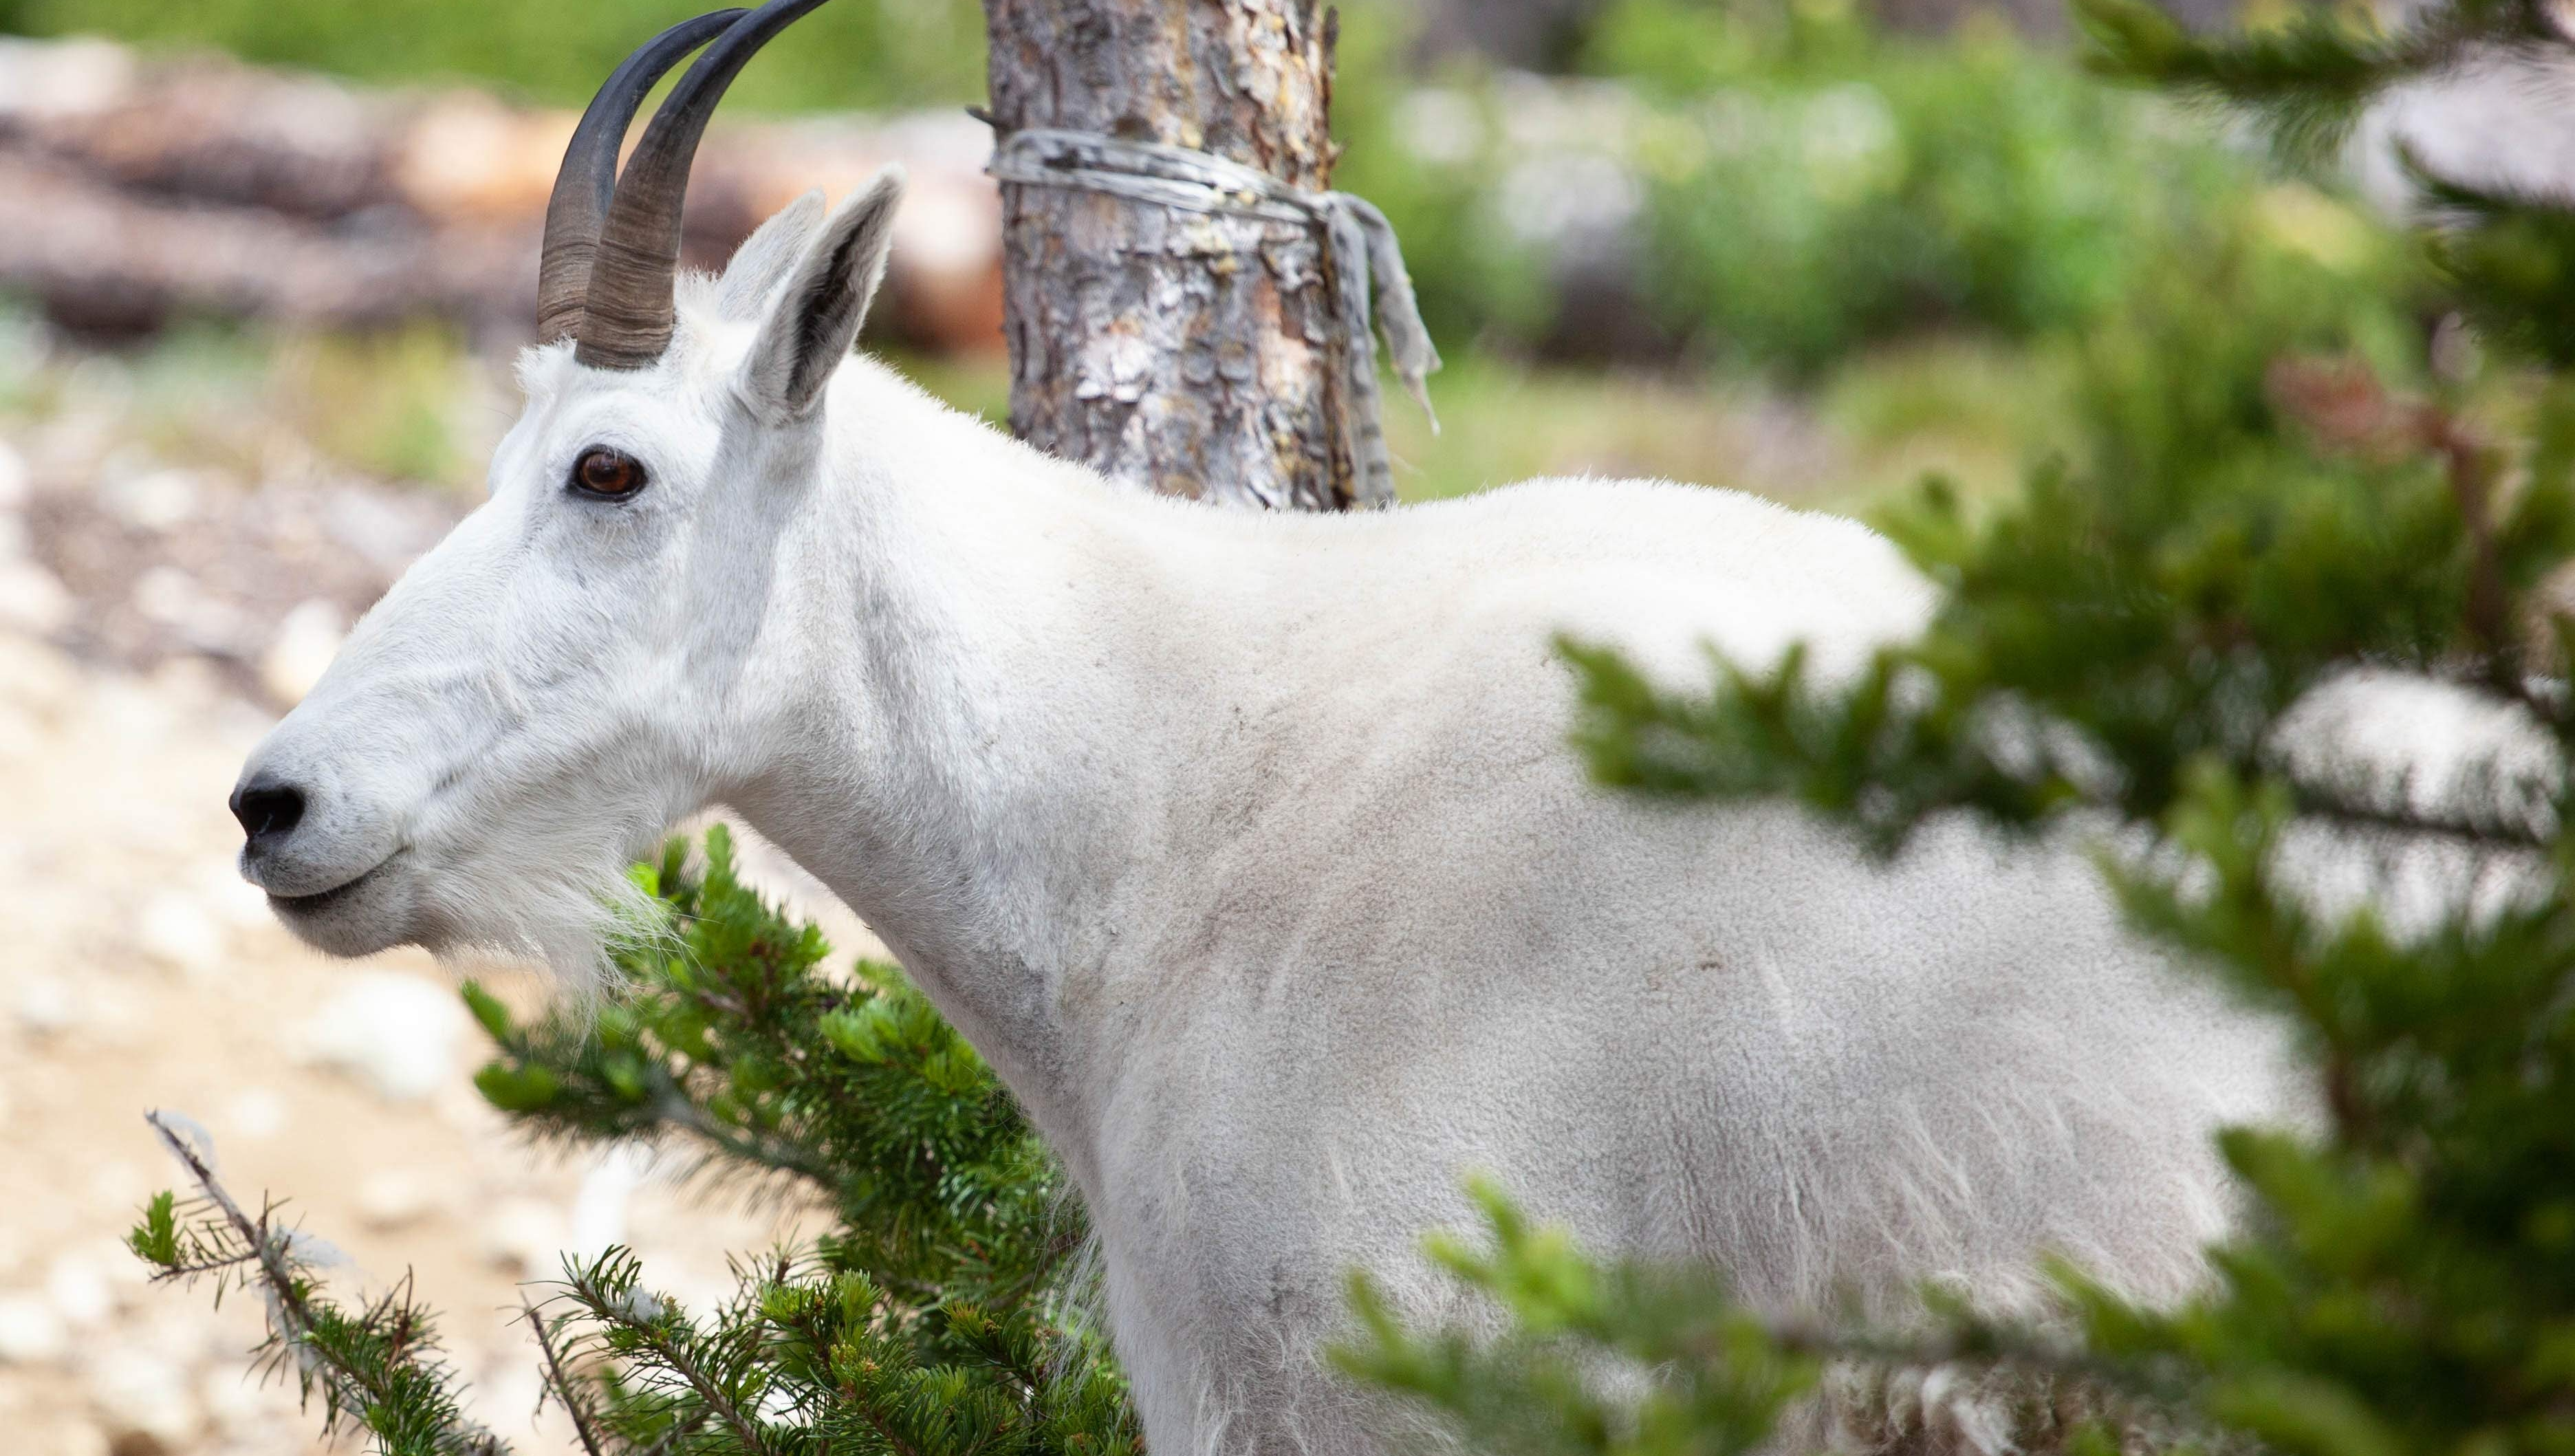
\includegraphics[width=\linewidth,keepaspectratio]{rectdummy}
  \caption{The conceptual picture of a control volume containing $n$ moving particles and $m$ resting particles. Migration in, entrainment, deposition, and migration out are represented by arrows, and the probability distribution of bed elevations is illustrated.}
  \label{fig:concept}
\vspace{-1.0cm}
\end{figure}

% link number of particles in motion to bedload transport
% link number of particles at rest to the bed elevation
The populations $n$ and $m$ link to the bedload transport rate $q_s$ and the bed elevation in the control volume.
The mean bedload transport rate $q_s$ is described by $q_s \propto u_s \bra n \ket$, where $u_s$ is the characteristic velocity of moving bedload and $\bra n \ket $ is the mean number of particles in motion \citep[e.g.][]{Charru2004, Ancey2008, Furbish2012a}.
To link the bed elevation $z$ to the number of resting particles $m$, we prescribe a mean number of particles at rest $m_0$ and introduce a packing fraction $\phi$ of grains in the bed.
Then from the bed geometry, considering a two-dimensional bed \citep[e.g.][]{Einstein1950, Paintal1971}, the deviation from the mean bed elevation is
\be z(m) = \frac{\pi a^2}{\phi L}(m-m_0) = z_1(m-m_0). \label{eq:ele}\ee
The constant $z_1 = \pi a^2/(\phi L)$ is an important scale of the problem. 
$z_1$ is the magnitude of bed elevation change (in an average sense across the control volume) associated with the addition or removal of a single particle. 

% develop the transition rates
% describe the markov property 
We write the rates for the four possible transitions as \citep[e.g.][]{Ancey2008}:
\begin{align}
 R_{MI}(n+1,m| n, m) &= \nu & \text{migration in}, \label{eq:rate1}\\
 R_E(n+1,m-1|n,m)  &= \lambda(m) + \mu(m) n  & \text{entrainment},  \label{eq:rate2}\\
 R_D(n-1,m+1|n,m) &= \sigma(m) n & \text{deposition},\label{eq:rate3}\\
 R_{MO}(n-1,m+1|n,m) &= \gamma n & \text{migration out\label{eq:rate4}}.
\end{align}
These rates are independent of the past evolution of the process, only depending on its current state $n,m$. 
This is the Markov hypothesis \citep[e.g.][]{Cox1965}, which implies the time intervals between subsequent transitions are exponentially distributed \citep[e.g.][]{Gillespie2007}.

% discuss the rates.
In these equations $\nu$ and $\gamma$, characterizing migration into and out of the volume are constants which do not depend on the populations $n$ and $m$.
In contrast, $\lambda(m)$, $\mu(m)$, and $\sigma(m)$, characterizing entrainment, collective entrainment, and deposition, respectively, depend on $m$.
Collective entrainment was introduced in \citet{Ancey2008} as a means to obtain bedload fluctuations of realistic magnitude and rectify some short-comings of an earlier work \citep{Ancey2006}.
This quantity has been discussed carefully in follow-up studies \citep[e.g.][]{Heyman2013, Heyman2014, Ma2014, Ancey2014a}, and we won't dwell on this topic.

% discuss the m dependence of the rates
The $m$ dependence in these transition rates is through the local bed elevation $z(m)$.
As is well-known, bed elevation changes modify the likelihood of entrainment and deposition \citep{Sawai1987, Wong2007}, meaning the entrainment and deposition rates depend on bed elevation.
\citet{Wong2007} concluded from their experiments that bed elevation changes induce an exponential variation in entrainment and deposition probabilities, while \citet{Sawai1987} concluded from his own experiments that the variation is linear.
For simplicity, we incorporate the scaling of \citet{Sawai1987} and note its equivalence to the \citet{Wong2007} scaling when bed elevation changes are small.

% set up the m dependence of the rates
This scaling can be written $\chi(m) = \chi_0(1\pm z_1 z(m)/(2l)^2)$, where $\chi = \lambda, \mu, \sigma$, and entrainment parameters take the plus sign while the deposition parameter takes the minus.
With these substitutions, the entrainment and deposition rates become:
\begin{align}
R_E(n+1,m-1| n,m)  &= (\lambda_0 + \mu_0 n)(1 + z_1z(m)/(2l)^2) + O(dt),\\
R_D(n-1,m+1| n,m) &= \sigma_0 (1-z_1z(m)/(2l)^2)n + O(dt).
\end{align}
In these equations, $l$ is a length scale of bed elevation change at which the entrainment and deposition rates are significantly affected, which we will clarify, and the ratio $z_1/l$ controls the sensitivity of these effects to the addition or removal of a single particle.
At $z(m)=0$, these reduce to the transition rates of the \citet{Ancey2008} theory.
Away from this elevation, entrainment and deposition are alternatively suppressed and accentuated, depending on the sign of $z(m)$, introducing a mean-reverting character to bed elevation changes.

% develop the master equation
In terms of the transition rates, we set up the Master equation describing the flow of probability through time as \citep[e.g.][]{Cox1965, Gillespie1992, Ancey2008}:
\begin{multline}
 \frac{\partial P}{\partial t}(n,m;t) =  
\nu P(n-1,m;t) + 
\{\lambda(m+1) + [n-1]\mu(m+1)\}P(n-1,m+1;t)\\ + 
[n+1]\sigma(m-1)P(n+1,m-1;t) + 
[n+1]\gamma P(n+1,m;t) \\- 
\{ \nu + \lambda(m) + n\mu(m) + n\sigma(m) + n \gamma \}P(n,m;t).
 \label{eq:master}
\end{multline} 
The solution $P(n,m;t)$ of this equation provides the statistics of $n$ and $m$, meaning it provides the statistics of bedload flux $q_s$ and bed elevation $z$ through equations \ref{eq:flux} and \ref{eq:ele}.
This equation represents a two-species stochastic birth-death model \citep[e.g.][]{Cox1965, Pielou1977} for the joint dynamics of bedload transport and bed elevations.

\section{Simulations}

% can't solve it analytically
% say why you chooes Gillespie
Equation \ref{eq:master} does not admit an analytical solution, at least by the methods applied to similar systems in the population ecology literature \citep[e.g][]{Swift2002}.
This difficulty is a consequence of the products between $n$ and $m$ in equation \ref{eq:master}.
In response to this, we proceed with numerical simulations.
The simulation of these birth-death type master equations has been extensively studied for its relevance to chemical physics and population ecology. 
Balancing conceptual simplicity against computational efficiency, we choose the classic and foundational Gillespie algorithm \citep{Gillespie1977, Gillespie1992, Gillespie2007}.

% explain Gillespie 
The Gillespie algorithm leverages the defining property of Markov processes: due to memorylessness in the rates \ref{eq:rate1}-\ref{eq:rate4}, the time interval between subsequent transitions is exponentially distributed \citep[e.g.][]{Cox1965}. Once a transition occurs, its type can be randomly selected using the relative rates of all possible transitions.
Accordingly, to step our birth-death process through a single transition, we can select the time to the next transition by drawing a random value from an exponential distribution, then we select the type of transition which occurs by selecting a random value from a uniform distribution. 
After this transition is enacted, i.e., by stepping $n$ and $m$ by the shifts associated with the type of transition which occurred, this two-stage selection is repeated indefinitely to form an exact realization of the stochastic process \citep{Gillespie1977, Gillespie1992, Gillespie2007}.
Computing the joint statistics of $n$ and $m$ from these simulations provides a numerical approximation of equation \ref{eq:master}.



\begin{wraptable}{l}{0.5\textwidth}
\caption{Parameters from \citet{Ancey2008} experiments describing the rates of migration in, entrainment, deposition, and migration out of the control volume when $z(m)=0$. All units are $s^{-1}$ (probability/time).}\label{tab:anceyparams}
\begin{tabular}{cccccc} \\ 
\toprule  
Flow & $\nu$ & $\lambda_0$ & $\mu_0$ & $\sigma_0$ & $\gamma$ \\
\midrule
(a) & 5.45  & 6.59  & 3.74 & 4.67 & 0.77 \\
\midrule
(g) & 7.74  & 8.42  & 4.34 & 4.95 & 0.56 \\
\midrule
(i) & 15.56 & 22.07 & 3.56 & 4.52 & 0.68 \\
\midrule
(l) & 15.52 & 14.64 & 4.32 & 4.77 & 0.48 \\
\midrule
(n) & 15.45 & 24.49 & 3.64 & 4.21 & 0.36 \\
\bottomrule
\end{tabular}
\end{wraptable} 
Using Gillespie's stochastic simulation algorithm, we simulated 5 flow conditions from the \citet{Ancey2008} experiments, prescribing 8 different values of the parameter $l$, ranging from half of the particle radius ($l=a/2$) to 4 particle diameters ($l=8a$) for a total of 40 simulations.
The parameters used for our simulations are taken from the experiments of \citet{Ancey2008} and are summarized in table \ref{tab:anceyparams}.
They are labeled (a), (g), and so on, in order of increasing bedload transport rate. 
Depending on the flow condition, exact stochastic trajectories consistent with equation \ref{eq:master} were simulated for either a $500$ hr or $1,000$ hr duration.
In all simulations, we take the packing fraction $\phi = 0.6$, a typical value for a pile of spheres \citep{Bennett1972}, and set $\Delta x = 22.5cm$ and $a = 0.3 cm$ in accord with the \citet{Ancey2008} experiments.

One simulated realization of our joint stochastic process for bed elevations and bedload transport is depicted in figure \ref{fig:pdfs} (a). 
These realizations determine the joint statistics of $n$ and $m$. 
The bedload transport statistics are depicted for a subset of all simulation conditions in figure \ref{fig:pdfs} (b). 
The \citet{Ancey2008} theory predicts negative binomial distributions for the number of moving particles within the control volume, and the mathematical form of these distributions is apparently not changed by our extension to account for feedbacks between bed elevation changes and entrainment and deposition probabilities.
We obtain an excellent negative binomial fit to the marginal probability distribution of $n$, $P(n) = \sum_m P(n,m,t)$, for all 40 of our simulation results.
However, particle activity statistics, including the mean particle activity and the variance of particle activity, are definitely shifted by the inclusion of differential mobility with bed elevation changes.
Bed elevation changes appear to buffer the magnitude of bedload fluctuations by up to 30 percent, which is an expected effect of the model, since a rapid increase in the bedload rate induced by a series of many entrainments will lower the bed elevation and increase the probability of deposition, buffering the magnitude of the bedload rate increase.

\begin{figure}[t!]
  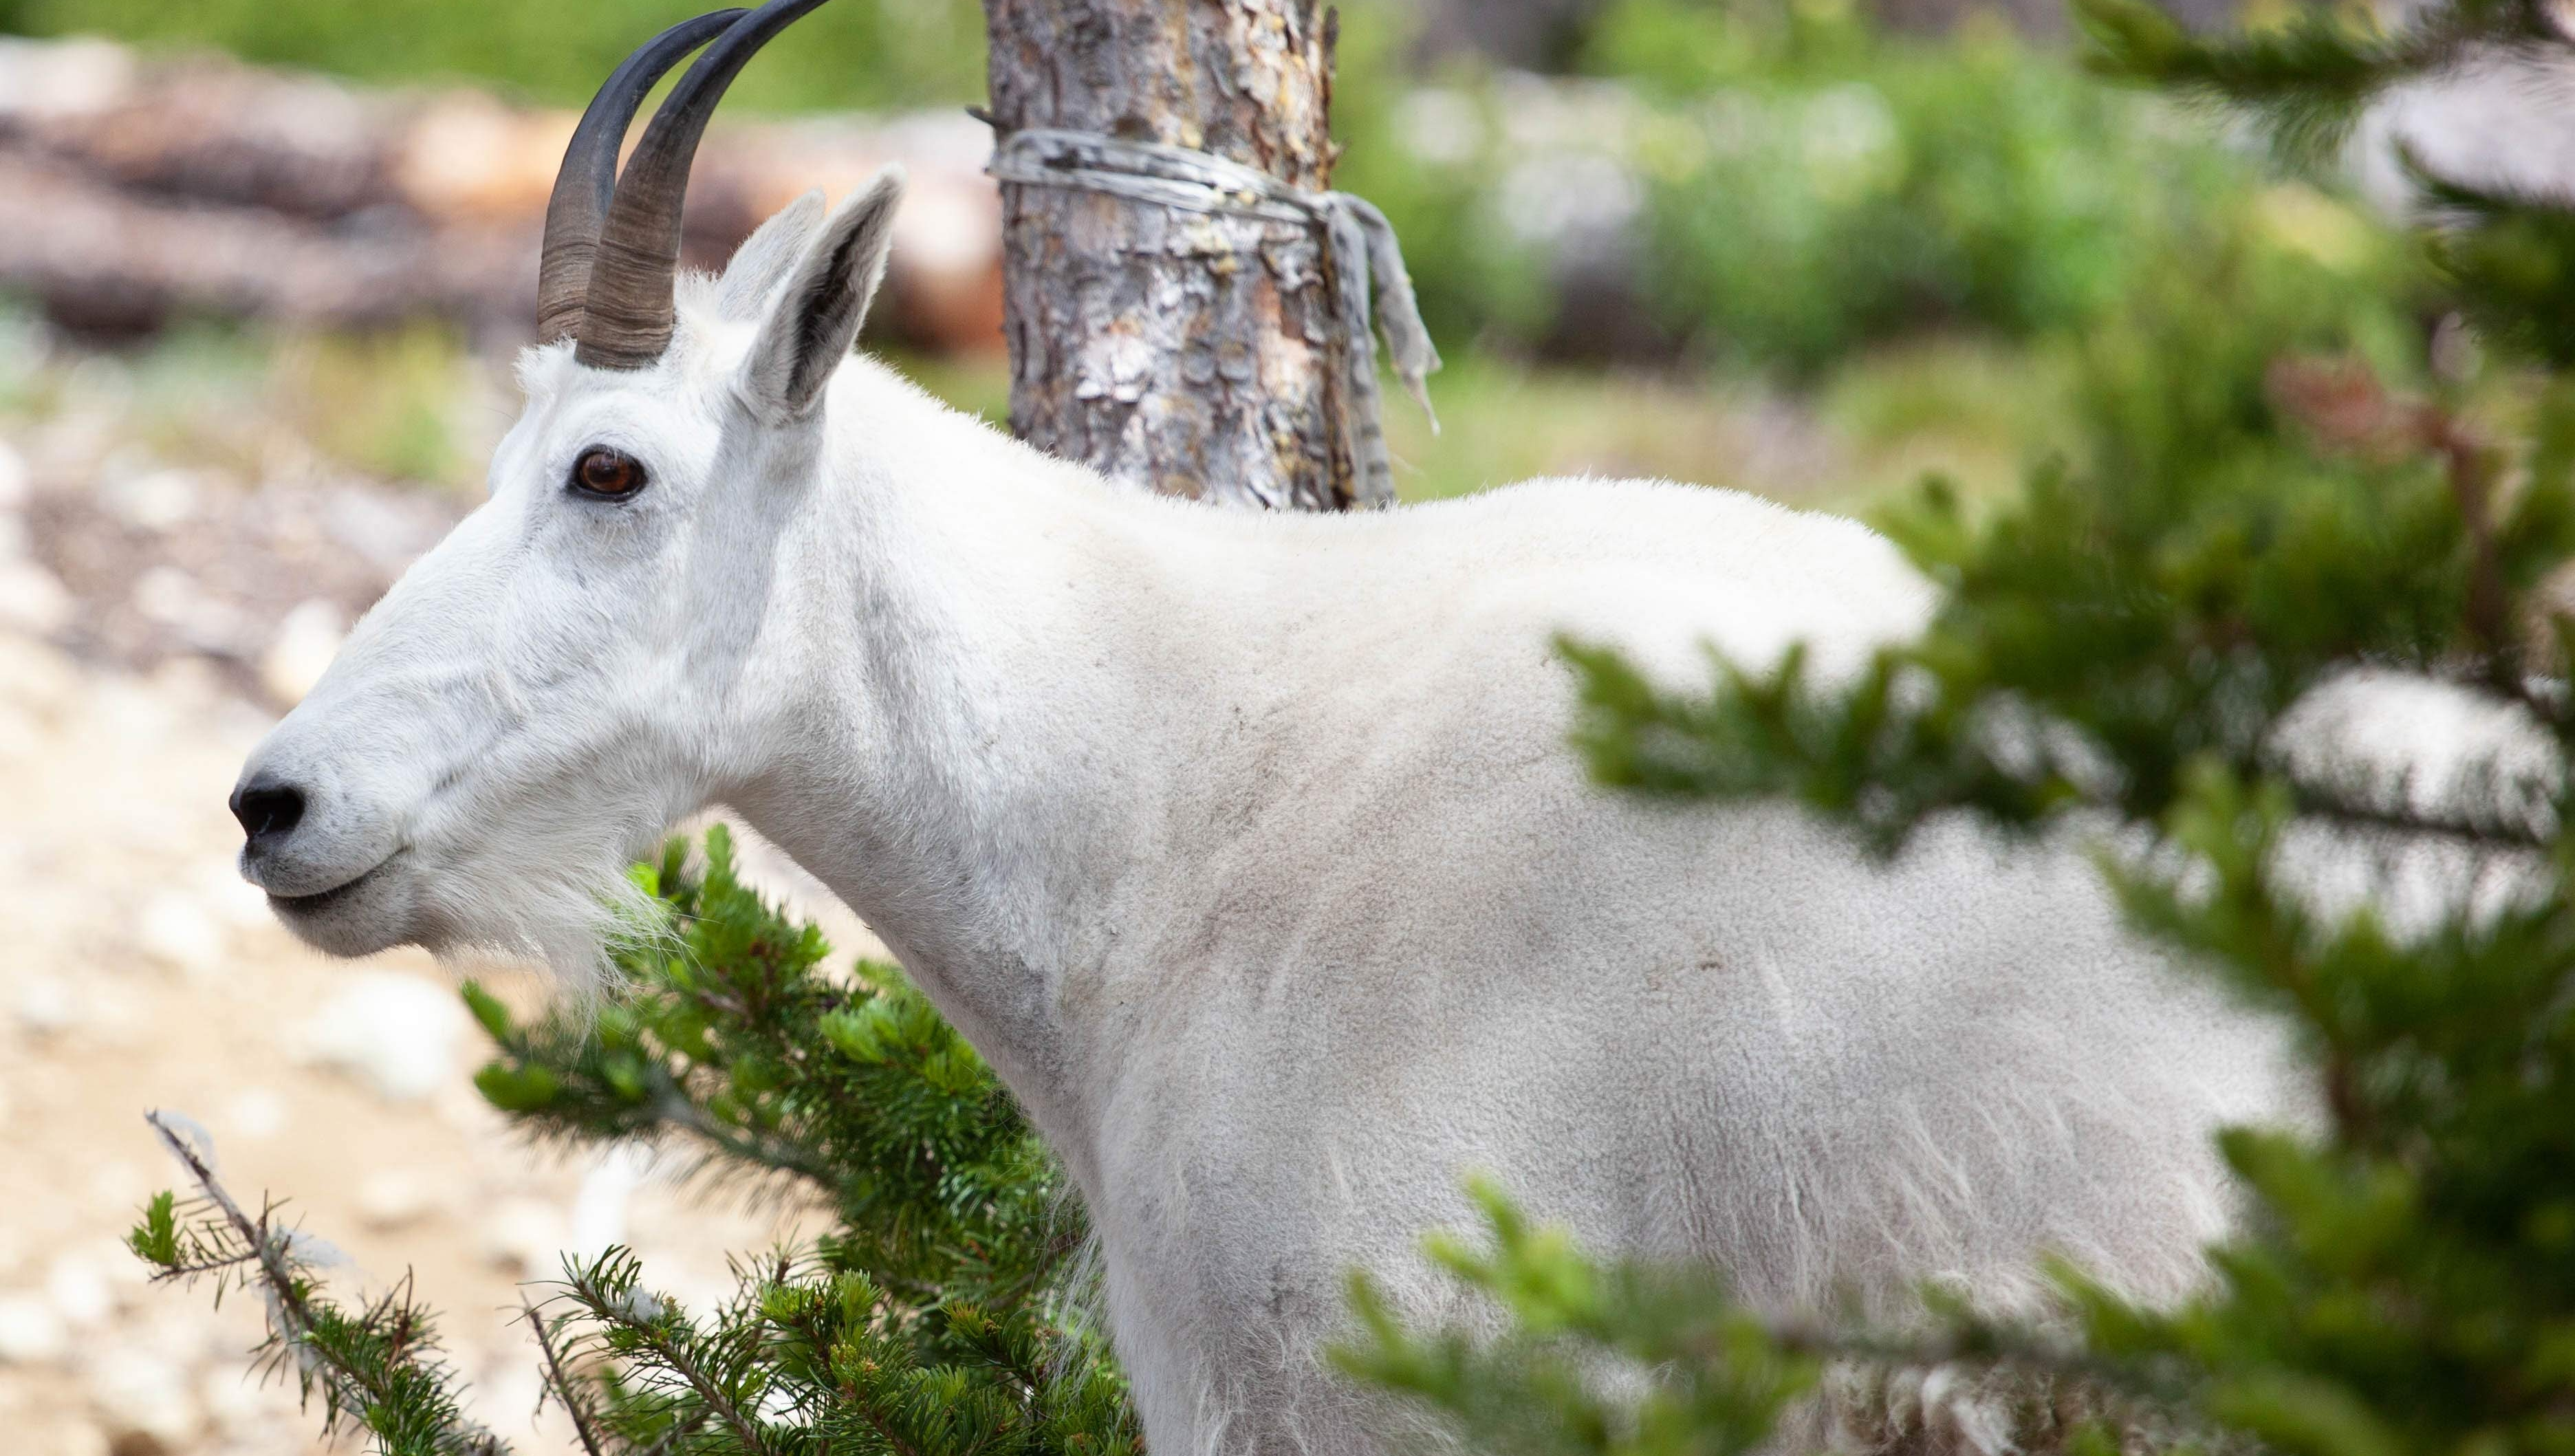
\includegraphics[width=\linewidth,keepaspectratio]{rectdummy}
  \caption{Figure (a) depicts timeseries of particle activity and bed elevation over a $20$ minute interval. Figures (b) and (c) display probability distribution functions of bed elevation (equation \ref{eq:ele}) and particle activity for a subset of the simulations. Colors represent flow conditions, while differing line styles represent different values of the differential mobility parameter $l$.}
\vspace{-1.0cm}
  \label{fig:pdfs}
\end{figure}

Our bed elevation timeseries exhibit longer temporal correlations than related bedload activity series, evident in figure \ref{fig:pdfs} (a). 
All 40 of our simulations develop clean unimodal distributions of bed elevations which are fit by Gaussian distributions with excellent correlation, and a subset of these marginal bed elevation pdfs with their Gaussian fits are displayed in figure \ref{fig:pdfs} (c). 
The mean number of particles resting on the bed is $m_0$, corresponding to a relative elevation $z(m_0)=0$. 
The variance of bed elevations is controlled by the differential mobility parameter $l$. 
Apparently, the simulations support the conclusion that $var(m) = (l/z_1)^2$. 
This conclusion is evident in figure \ref{fig:var}, with generally excellent correpsondence between this relationship and the simulation points, with some scatter we attribute to the finite duration of our simulations.

To compute the resting time distribution; at each elevation $m$, we extract the set of all departure times from this elevation, or times at which the bed was at this elevation and a deposition occurred; then we extract the set of all return times to this elevation, or times at which the bed was one increment above this elevation ($m+1$) and an entrainment occurred.
Taking differences between these two time-series returns the set of all return times from above marginal to the elevation $m$, which we binned across a $0.5$s interval to compute the cumulative probabilities of return times at each elevation m, $P(T_r>t|m)$.
Following earlier investigators, we computed the unconditional or over-all rest time distribution as the convolution of these conditional distributions over all bed elevations \citep[e.g.][]{Yang1971, Voepel2013}:
\be P(T_r>t) = \sum_m P(m) P(T_r > t| m), \ee
where $P(m)$ is the pdf of bed elevation like those depicted in figure \ref{fig:pdfs} (b) and the sum is over all bed elevations attained during the simulation. 

\begin{wrapfigure}{r}{0.5\textwidth}
\centering
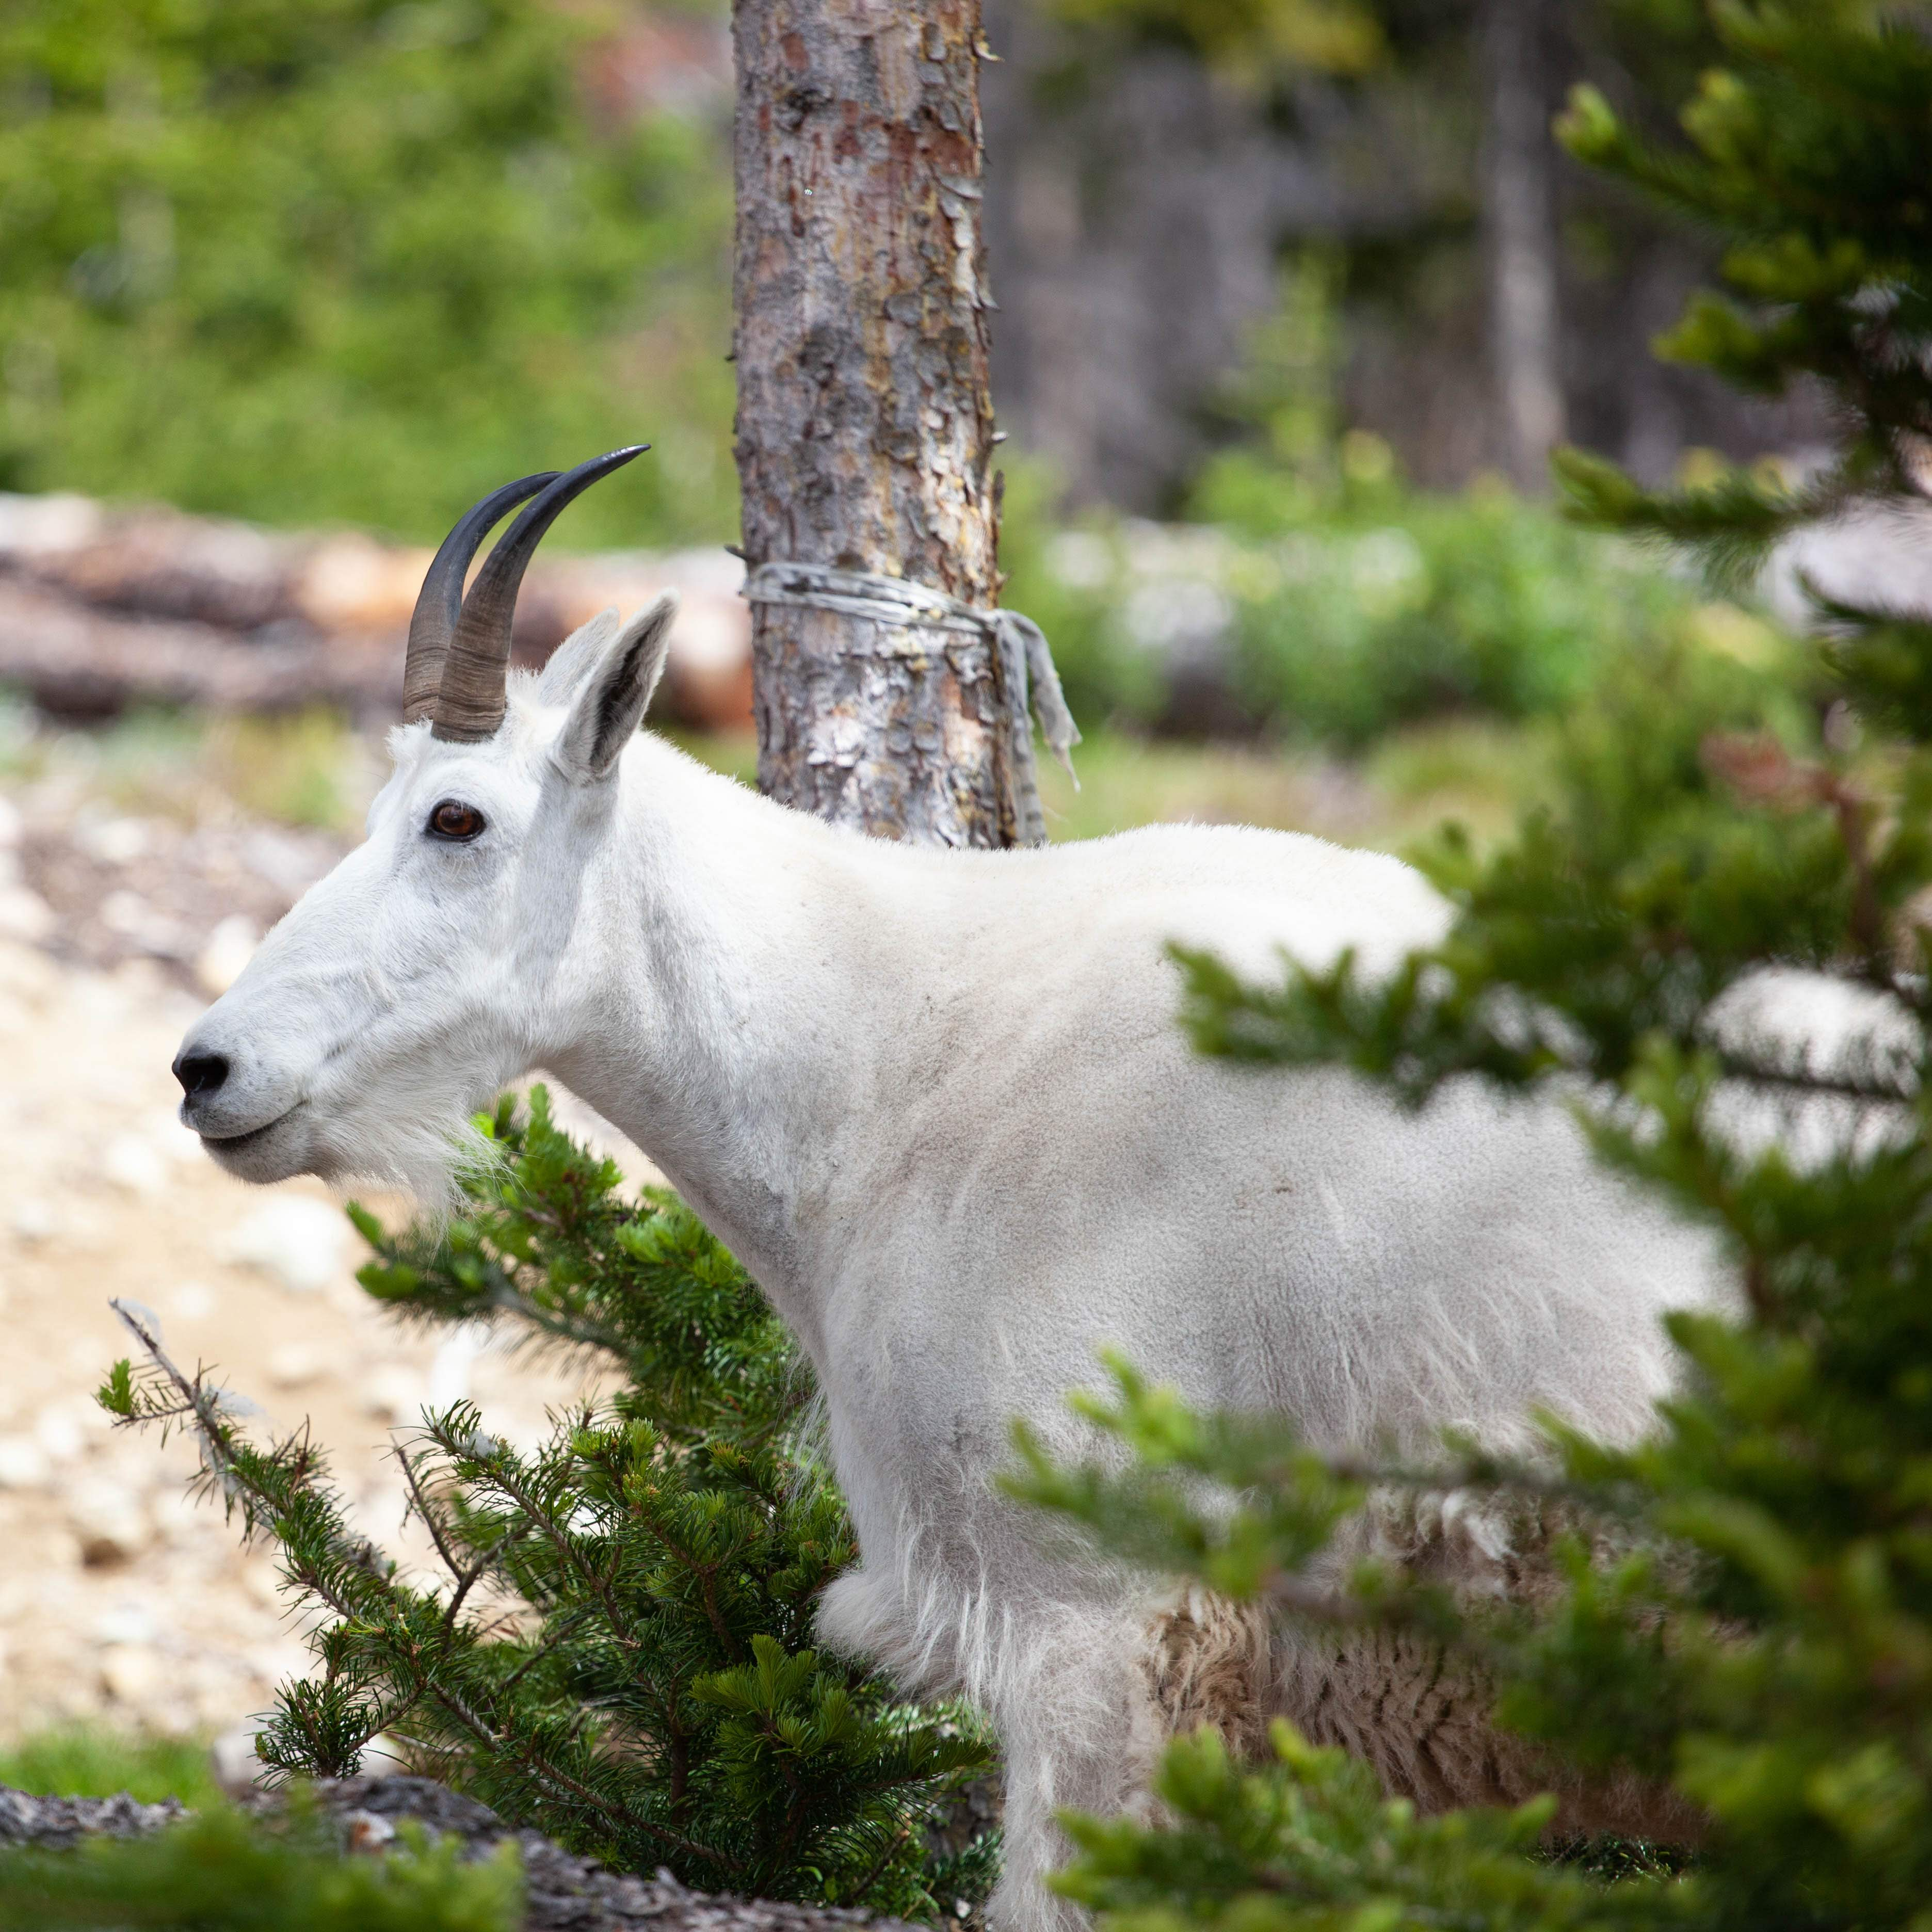
\includegraphics[width=0.5\textwidth,keepaspectratio]{squaredummy}
\caption{The standard deviation of bed elevation scales one-to-one with the differential mobility parameter $(l/z_1)$, indicating the ratio $l/z_1$ controls the magnitude of bed elevation fluctuations. }
\label{fig:var}
\end{wrapfigure}

This analysis derives unconditional exceedance probabilities of resting times with heavy power-law tails. 
A subset of all of our simulation results are depicted in figure \ref{fig:collapse} (a)-(d). 
Apparently, for suitably long times, the tail parameter $\alpha$ of these resting time distributions is independent of flow conditions or the differential mobility parameter $l$. 
However, the timescale at which particle resting transitions from exponential to power-law scaling shifts with flow conditions and $l$. 
\citet{Martin2014} obtained an approximate collapse at the tails of their experimental resting time distributions using the reciprocal of the rate of entrainment or deposition events occurring. They denoted this rate by $a$, so that their timescale was $1/a$.
Scaling the resting times by $1/a$ provides an incomplete collapse of the tails of our simulated resting time distributions, which may describe the incomplete collapse of the experimental data of \citet{Martin2014}.  
It collapses the tails across flow conditions when $l$ (the standard deviation of bed elevation) is fixed, i.e., it leads to the collapse seen between figures \ref{fig:collapse} (a) and \ref{fig:collapse} (b), but if $l$ (which is the standard deviation of bed elevation) varies with flow, then the power-law scaling of resting times is no longer controlled by $1/a$ alone. 
Instead, we must include a factor representing the differential entrainment and deposition characteristics of grains as the bed elevation changes. 
The timescale which provides universal collapse of the power-law tails of all our simulations is $T_0 = l/(z_1E),$ where $E$ is the entrainment rate.

\begin{figure}[t!] % t for top and ! for force it 
  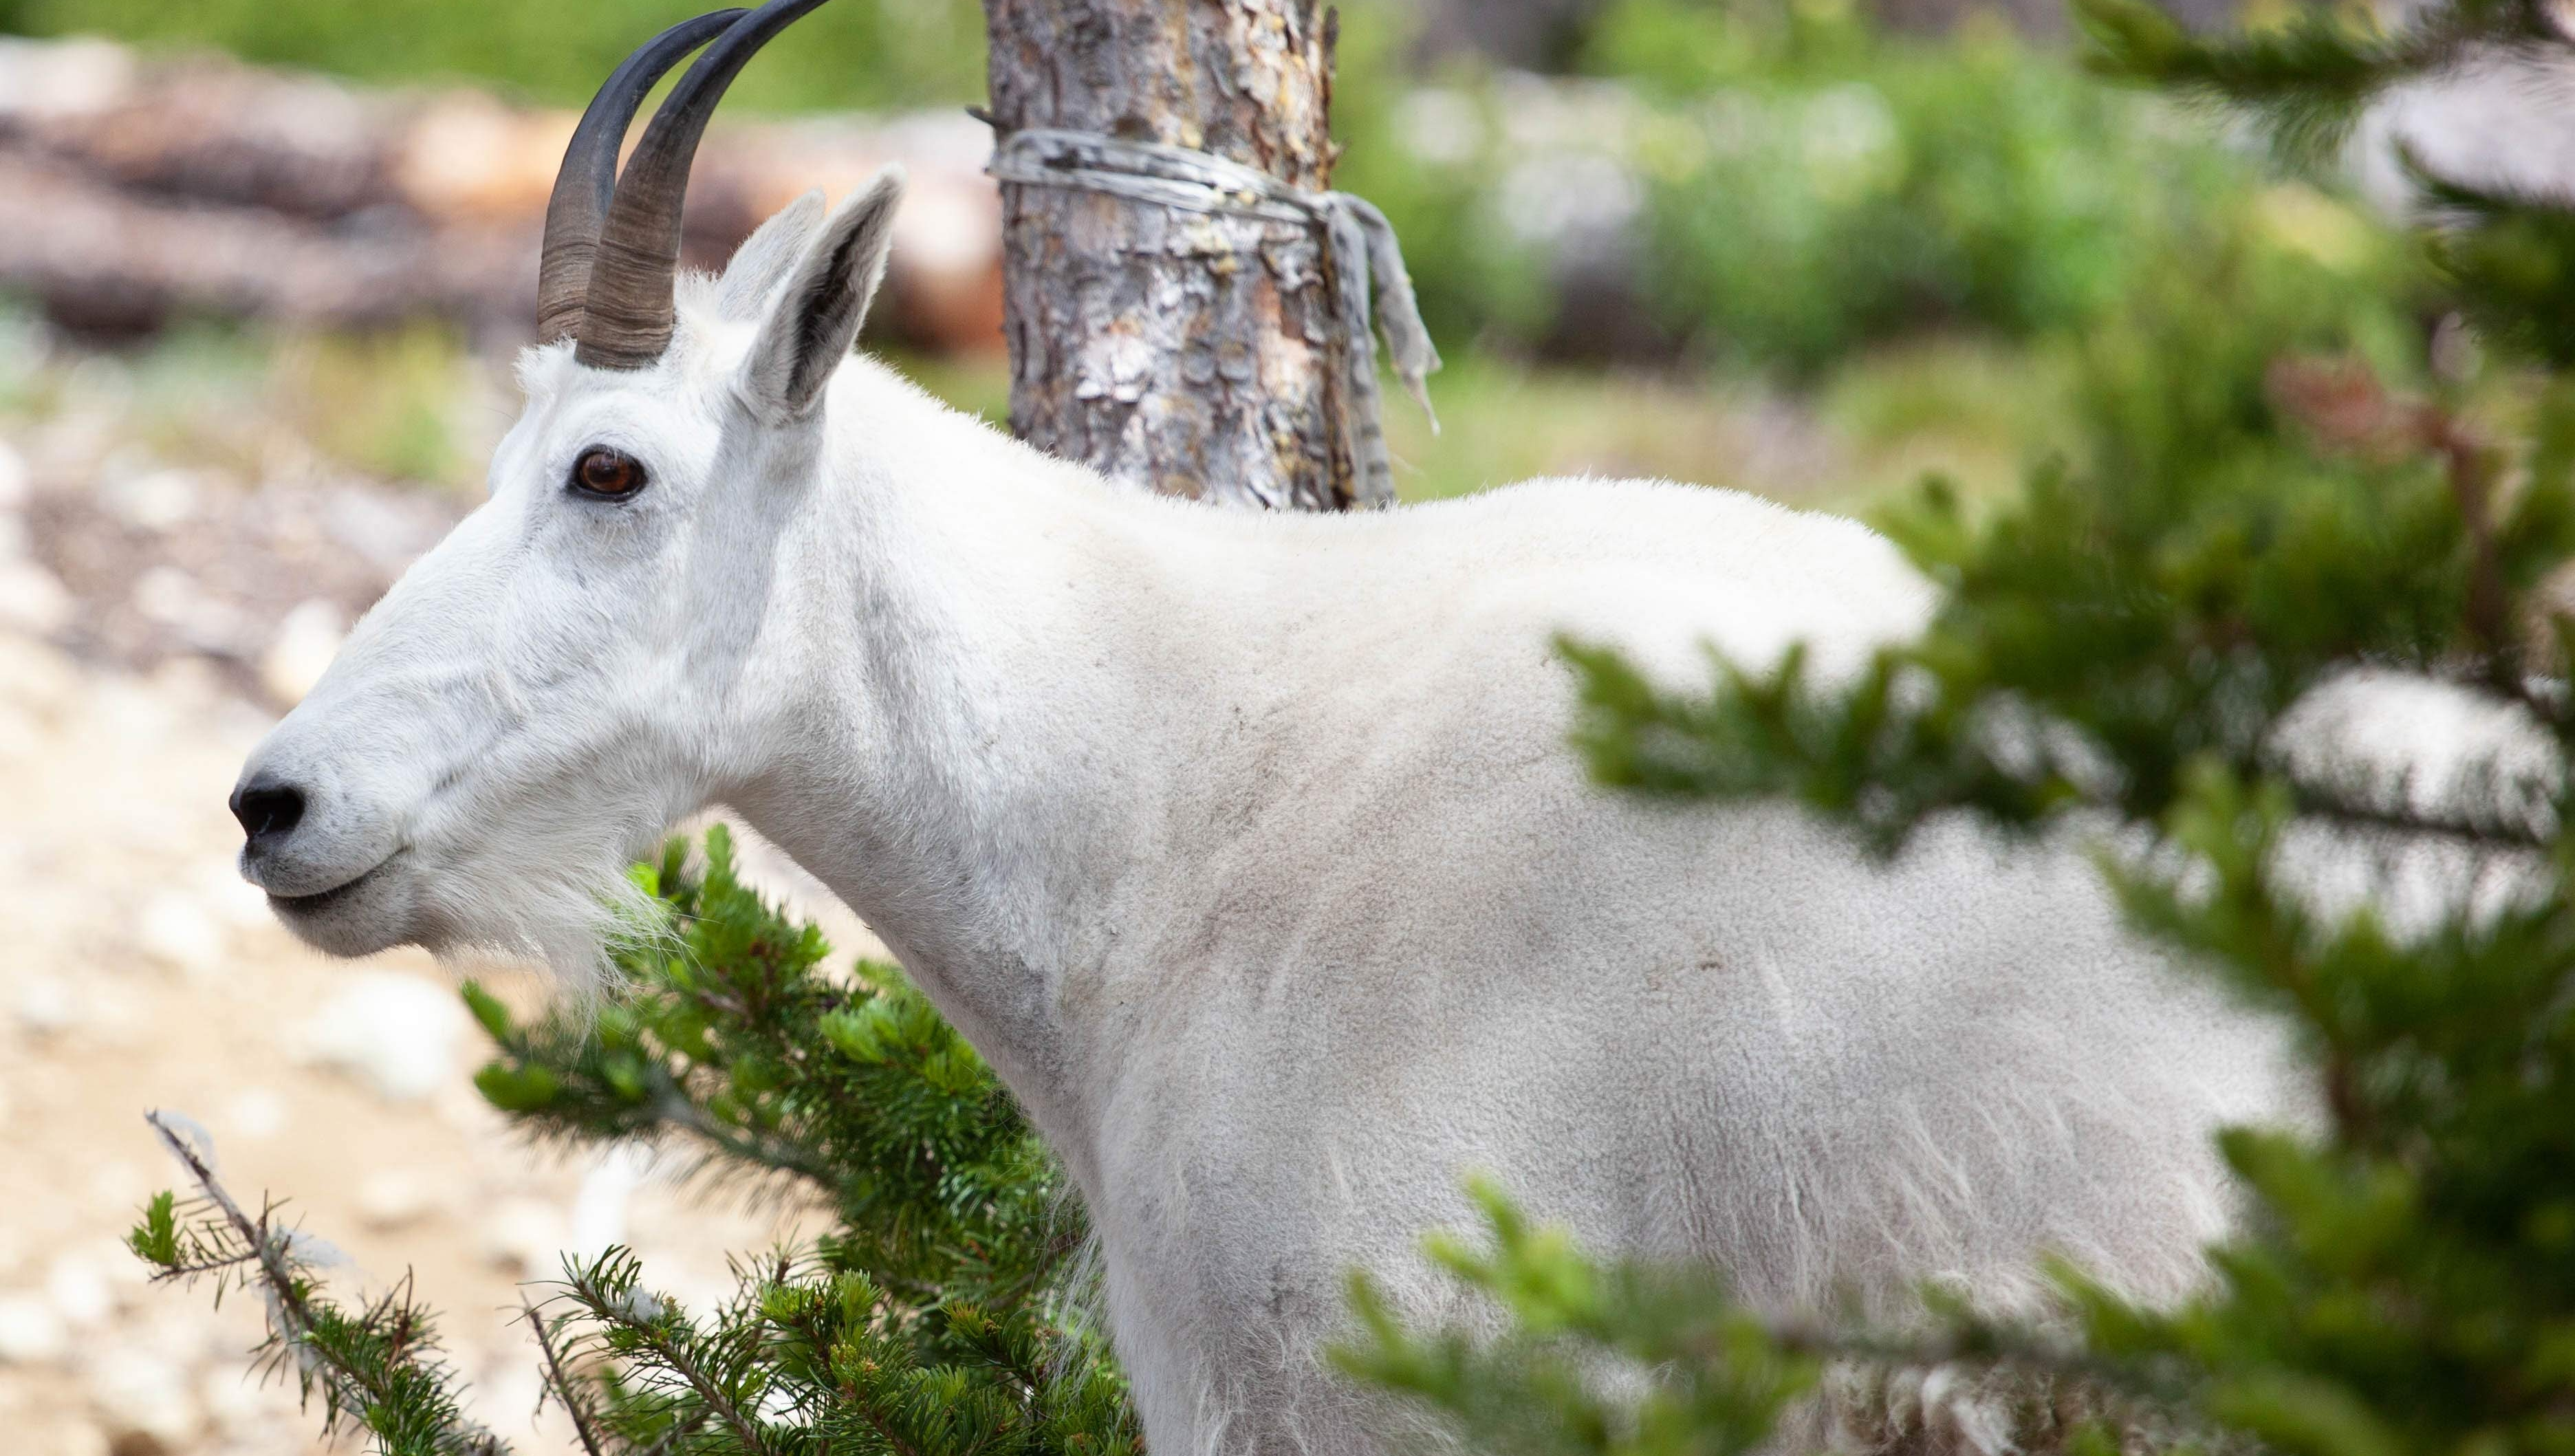
\includegraphics[width=\linewidth,keepaspectratio]{rectdummy}
  \caption{This figure summarizes the resting time exceedance distributions for a subset of all simulations. Part (a) displays resting time distributions for a range of flow conditions at fixed $l$, while part (b) displays the collapse obtained by scaling $T_r$ by $T_0$. The collapse between (a) and (b) is analogous to \citet{Martin2014}, and it is induced by the factor of $1/E$ within $T_0$. Parts (c) and (d) display a similar collapse for a fixed flow condition at variable $l$. In this case, collapse is driven by the factor of $z_1/l$ within $T_0$, and this influence of differential mobility in resting statistics has not to our knowledge been noticed up to now.}
\vspace{-1.0cm}
  \label{fig:collapse}
\end{figure}

We can understand $T_0$ with a physical argument.
According to figure \ref{fig:var}, the typical length scale of bed elevation fluctuations is $l$, and as mentioned the length scale $z_1$ is the magnitude of bed elevation change enacted by the entrainment or deposition of a single particle.  
In equilibrium bedload transport, \citet{Einstein1950} tells us the condition $E=D$ holds: this is a statement of mass conservation. 
Since $E$ represents the mean number of particles removed from the bed in a unit of time, the product $E z_1$ can be interpreted as a representative velocity scale of bed return. 
It is the distance the bed lowers with the removal of a single particle divided by the mean time required to remove it.
Hence we extract our timescale as a key distance scale over a key velocity scale: $T_0 = l/(z_1 E).$ 
Scaling the resting time as $T_r/T_0$ exhibits a consistent power-law tail across all of our simulation results. 

\section{Discussion}

Our theory of bed elevations derives results similar to \citet{Martin2014} using bedload transport as a starting point, and it also provides a statistical characterization of bedload transport.
Our assumptions derive a heavy-tailed power-law distribution of resting times with a tail parameter $\alpha \approx 1$ which displays differences across flow conditions which partially collapse upon scaling by an activity timescale.

However, in extension of the \citet{Martin2014} theory, our model reveals another timescale which fully collapses the power-law tails of the resting time distributions, suggesting a universal power-law should characterize the asymptotic resting times of sediment undergoing burial if the assumptions of our model are correct.
This timescale includes an additional factor characterizing the dependence of entrainment and deposition probabilities on changes in local bed elevations.
We hypothesize this new factor may explain some of the differences between field \citep[e.g.][]{Olinde2015} and laboratory \citep[e.g.][]{Martin2014} observations of resting time distributions, providing additional information to determine whether burial is the dominant mechanism of the heavy-tailed sediment resting times observed in natural channels.


Pierce
The model describes why Martin et al (2014) obtained incomplete collapse between their resting time distributions. They didn't include the $(z_1/l)^2$ type factor in their scaling time-scale
It is a first joint stochastic description of bed elevations and bedload transport, mixing martin 2014 and ancey 2008. 
It provides a mechanism for heavy-tailed resting times and implies super-diffusion of bedload and a virtual velocity of sediment which decreases toward zero with time. 
 what else? help



Hassan
1.      Discuss what is special in the model and how it works. (most of point number 2)

2.      Your point number 1

3.      The last pargraph from the introduction

4.      Your point number 3 with implications (What this means for the study of bedload (and channel morphology in streams). The implications should be short.


\section{Conclusion}
\begin{comment} 
Bedload diffusion is anomalous because of heavy-tailed sediment resting times \citep{Bradley2017}.
Several theories have shown that heavy-tailed resting times should result from sediment burial \citep{Voepel2013, Martin2014}, and a few experiments have resolved heavy-tailed resting times within natural channels \citep{Olinde2015, Bradley2017}, but these experiments do not support a consensus on the power-law decay, truncation properties, or scaling behavior of the resting time distribution.
Bedload transport and bed elevations vary randomly, so we have pursued a joint stochastic model of these quantities based on a juncture of earlier works \citep{Ancey2008, Martin2014}.
Following the classic literature to interpret burial times as the return time from above in the bed elevation time series \citep{Yang1971, Nakagawa1980}, and including the effect of mobility variation with local bed elevation changes \citep{Sawai1987, Wong2007, Martin2014}, we obtained at a few key conclusions regarding the resting time of sediment undergoing burial.
 
First, particle activities lie on negative binomial distributions, meaning they exhibit relatively wide bedload transport fluctuations. 
This result is essential unchanged from the \citet{Ancey2008} theory, except the moments of the particle activity distribution do shift as a result of bed elevation changes. 
In this work we have chosen to neglect this topic to support a more careful discussion of resting times, but this observation of a negative feedback between bedload fluctuations and bed elevation changes is worth a more careful analysis. 
Second, bed elevations lie on Gaussian distributions, reflecting symmetrical variations in bed elevations, and thin tails which suppress but do not prohibit extreme bed elevation variations.  
Third, and most importantly, the resting time of stationary sediment undergoing burial lies on a heavy-tailed distribution which decays as a power-law with tail parameter $\alpha \approx 1.0$. Our resting time distributions are truncated at a timescale related to the period of observation, and we uncover universal scaling in the power-law decay of these distributions by the timescale $T_0 = l/(z_1E)$.

The timescale $T_0$ is derived from a physical argument: it is the ratio of the representative length scale of bed elevation variations $l$ with a velocity scale of bed elevation changes $z_1 E$. 
Conceptually, $1/E$ is equivalent to the timescale $1/a$ used by \citet{Martin2014} to attain a partial collapse of their resting time distributions across various flow conditions.
Actually, the rate $a$ of entrainment or deposition occurring is $a \approx E+D$, and in equilibrium bedload transport we have $E\approx D$ \citep{Einstein1950}, so $E = a/2$. 
To fully collapse our simulated resting time distributions, the timescale $1/E$ is not sufficient: it collapses across variations in flow but it does not collapse the power-law tails across the concordant variations in the magnitude of bed elevation fluctuations ($l$).
This observation suggests the incomplete collapse of the power-law resting time tails of the \citet{Martin2014} flume experiments, and the appreciable variability of the \citet{Olinde2015} field experiments might be attributed to the differential mobility of bed particles with bed elevation changes, which our model encodes in the ratio $l/z_1$.

In conclusion, we highlight that sediment burial under a region of bed under-going active bedload transport, as we have modeled here, is probably only one mechanism from which natural rivers might express the heavy-tailed sediment burial time distributions which have been observed in tracer experiments \citep{Voepel2013, Olinde2015,Bradley2017}.
The resting time distributions we have simulated, although they have satisfying correspondence with the laboratory experiments of \citet{Martin2014}, where heavy-tailed resting times are verifiably controlled by burial, have limited explanatory power over the excellent field data of \citet{Bradley2017}, which were obtained from a 9 year series of tracer observations.
In natural channels, other mechanisms may induce heavy-tailed resting times of sediment: \citet{Bradley2017} suggested we might look to other stochastic return processes within fluvial channels, such as the return of water levels to tracer particles stranded high on a bar, to gain understanding of sediment resting times.
Similarly, \citet{Malmon2005} suggested sediment residence within floodplains is controlled by the timescales of river channel migration, meaning the resting times of sediment really link to a host of processes from the compounded timescales of individual granular movements, like we have modeled, up to intermediate timescales related to the intermittency of floods, as suggested by \citet{Bradley2017}, all the way up to morphological timescales such as those characterizing channel migration.

Probably, for considerations of contaminant evacuation from gravel bed rivers on typical timescales of ecological relevance (decadal, centennial), a predictive understanding of sediment resting will require the former two processes: sediment burial and water level return. 
In this work, we hope we have created new understanding of the former, uncovering some universal scaling properties.  
The latter topic, which was suggested by Bradley but has not yet been studied, deserves immediate research attention.
According to our model, sediment burial alone is enough to induce fluvial sediment resting time distributions with heavy tails sufficient to drive an arbitrary slowdown of tracer particles or solid contaminants as their period of residence in the channel is increased, and we can state confidently that under idealized conditions when the assumptions of \citet{Einstein1950} are valid, this heavy-tail will decline approximately as $P(T_r) \propto (T_r/T_0)^{-1}$, but we have no idea how these conclusions would be modified by multiple return processes acting in concert, although we hypothesize this could explain the relatively slower decays seen in field data, for example the values of $0.31<\alpha<0.72$ of the \citet{Olinde2015} experiments.
We hope to see subsequent theories deriving resting times from more general channel return processes acting in coordination, and a proliferation of experiments, so we can pin down a mechanistic theory of anomalous diffusion and fluvial contaminant transport.
\end{comment}
\acknowledgments
The computer code used to simulate the presented model is available upon request from the authors.
Marwan A. Hassan is funded by xxx. James K. Pierce is funded by yyy. The authors benefited from conversations with Shawn Chartrand and Conor McDowell. 

\bibliography{biblio}

\end{document}




